%%%%%%%%%%%%%%%%%%%%%%%%%%%%%%%%%%%%%%%%%%%%%%%%%%%%%%%%%%%%%%%%%%%%%%%%%%%%%%%%%%%%%%%%%%%
%%
%% The updated version of this document should be downloaded from
%%      https://github.com/jp-um/university_of_malta_LaTeX_dissertation_template
%%
%% In case of any difficulties please contact Dr JP Ebejer on jean.p.ebejer@um.edu.mt
%%
%%%%%%%%%%%%%%%%%%%%%%%%%%%%%%%%%%%%%%%%%%%%%%%%%%%%%%%%%%%%%%%%%%%%%%%%%%%%%%%%%%%%%%%%%%%

%% Before you embark on this quest you should probably read some of:
%% Deadly sins - http://mirrors.ctan.org/info/l2tabu/english/l2tabuen.pdf
%% Writing a thesis in LaTeX - http://tug.org/pracjourn/2008-1/mori/mori.pdf

\RequirePackage[l2tabu, orthodox]{nag} % tells you of any bad LaTeX usage
                                       % must be first thing in class (with the exception of comments)

%% There is one option you should define; oneside or twoside
%% Use twoside for your viva docs (examiners hate long docs they need to carry around)
%% and oneside for the final thing you submit to the library.  Note that margins will
%% change accordingly

\documentclass[twoside]{um}  % custom University of Malta project/dissertation/thesis 


%% **************** (Your) Packages (Start) ******************

% \listfiles % uncomment this to know which packages you are using
              % the list of packages will be in the bottom of the .log file

%% Note that packges may already be loaded from the um (and memoir) classes.
%% Do not add your packages to the template, but rather add them here.

\usepackage{blindtext} %% for some dummy text, remove in your writeup
\usepackage{coffee4}    %% for some fun
\usepackage{amsmath} %% line breaks equation
\usepackage{float}

%% ***************** (Your) Packages (End) *******************


%% **************** (Your) Data (Start) ******************

\title{Machine Learning for the Prediction of Brake Bending Parameters}  % use \\ here otherwise you get a justified title
                                     % note capitalization of the title (only common 
                                     % words in lower case)
\tagline{some hyped-up tagline}      % tag line
\author{Philipp Kurrle}            % your full name
\authorID{123456}                   % your University Identifier
\supervisor{Prof. Dr. Ulrike Pado}              % your supervisor(s) name - no . in Dr
\cosupervisor{Peter Lange}                % your cosupervisor(s) name - no . in Dr *OPTIONAL* 
\university{Hochschule für Technik}

                                     % simply comment out the above line if absent
\department{Computer Science}   % your department (e.g. Artificial Intelligence)
\faculty{Software Technology Master}       % your faculty (e.g. ICT)
\degreeName{M.Sc.\ in Software Technology}       % the degree you are reading
                                     % note the \ after the dot, so not to consider it a fullstop
\doctype{dissertation}               % the type of document (fyp, dissertation, thesis)
\degreeDate{\monthyeardate\today}    % when did you submit (officially after your corrections)
%%\subjectcode{ICS5200}                % the study unit-code (currently not used)

%% ***************** (Your) Data (End) *******************

%%
\renewcommand{\chapterheadstart}{\vspace*{\beforechapskip}}
\setlength\beforechapskip{0mm}



%% ******** (Your) Document Settings (Start) *************

% You should have an images directory in every chapX subdir
% NOTE:  Trailing / for subdirs is required.
\graphicspath{{./images/}{./chap1/images/}{./chap2/images/}{./chap3/images/}}   % Paths where to look for images, if defined "images" must always be there as it holds the images in-use by the template.

\makeindex

%% ********* (Your) Document Settings (End) **************

% DOCTOR'S (JP) ORDERS: MAKE SURE TO READ MY TWO BLOG ENTRIES WITH
% CONTENT AND LaTeX TIPS FOR YOUR WRITE-UP.  THESE ARE BASED ON  
% EXAMINER'S FEEDBACK
%
% URLS:
% https://bitsilla.com/blog/2019/03/content-tips-for-your-dissertation-or-project-write-up/
% https://bitsilla.com/blog/2019/01/latex-tips-for-your-dissertation-or-project-write-up/

% end the preamble and start the document

\begin{document}
\frontmatter 
    \maketitle
    %\input{frontmatter/copyright}       
    %% The originality statement is *NOT* part of the dissertation but submitted separately.
    %\input{frontmatter/dedication}        % include a dedication.tex file
    %\input{frontmatter/acknowledgements}   % include an acknowledgements.tex file
    \input{frontmatter/abstract}\if@openright\cleardoublepage\else\clearpage\fi
    \tableofcontents*\if@openright\cleardoublepage\else\clearpage\fi
    \listoffigures*\if@openright\cleardoublepage\else\clearpage\fi
    \listoftables*\if@openright\cleardoublepage\else\clearpage\fi
    \input{frontmatter/abbreviations}\if@openright\cleardoublepage\else\clearpage\fi

%% Note: always use \input as you cannot nest \includes (amongst other things)
\pagestyle{umpage}
\floatpagestyle{umpage}
\mainmatter 
%%	\part{Your First Part} %% PhDs may require this parts idea as well.
    \chapter{Introduction}

Note that you may have multiple \texttt{{\textbackslash}include} statements here, e.g.\ one for each subsection.

General structure of this chapter should read as follows.  This chapter should be used to motivate your study and answer the question ``Why is this important?''. Also, it should define what you set out to achieve (these will be revisited in the conclusions chapter). You should describe your approach to the Aims and Objectives, including an evaluation part. \cofeBm{1}{1}{0}{4cm}{-3cm} %% coffee mark HA HA!

\section{Motivation} % why is this a non trivial problem
\blindtext

\section{Aims and Objectives} 
\blindtext

\section{Our Approach} 
\blindtext

\section{Document Structure}
\blindtext
 
    %\chapter{Background \& Literature Overview}

In this section you need to explain all the theory required to understand your dissertation (i.e.\ the following chapters). But really in this chapter I am going to show you some examples.

\section{An Example of an Equation}

The following is the most beautiful equation in maths, Euler's Identity (Equation~\ref{eq:euleridentity}).

\begin{equation}\label{eq:euleridentity}
	e^{i\pi}+1=0
\end{equation}
where:
\begin{conditionsenv*}
	e 		& the constant \\
	i 		& of complex fame \\
	\pi		& not of the apple variety \\
\end{conditionsenv*}

\blindtext[2]

\section{An Example of a Numbered List}

This is an example of a numbered list:

\begin{enumerate}
	\item This is my first point
	\item My second
	\item My third!
	\item And my fourth?
\end{enumerate}

\blindtext

\section{An Example of a Bulleted List}

This is an example of a bulleted list:

\begin{itemize}
	\item This is my first point
	\item My second
	\item My third!
	\item And my fourth?
\end{itemize}

\blindtext

\section{An Example of a Figure}

A test figure is shown in Figure~\ref{fig:test1}.

\begin{figure}[ht!] % supposedly places it here ...
	\centering
	\includegraphics[width=0.6\linewidth]{test_image_goku}
	\caption[This is the short caption for List of Figures]{A test figure.  This caption is huge, but in the list of figures only the smaller version in the square brackets will appear.\index{Goku il-king}}
	\label{fig:test1}
\end{figure}

\blindtext

\section{An Example of a Side-by-Side Figure}

Two figures shown side-by-side are shown in Figure~\ref{fig:test2}.

\begin{figure}[!ht]
	\centering
	\subbottom[Goku]{\includegraphics[width=0.3\textwidth]{test_image_goku}}\qquad
	\subbottom[More Goku]{\includegraphics[width=0.3\textwidth]{test_image_goku}}%
	\caption[Short Caption]{The same super saiyan. Two times.}        
	\label{fig:test2}
\end{figure}

\blindtext

\section{An Example of Using Acronyms}

In the early nineties, \acs{GSM} was deployed in many European countries. \ac{GSM} offered for the first time international roaming for mobile subscribers. The \acs{GSM}’s use of \ac{TDMA} as its communication standard was debated at length. And every now and then there are big discussion whether \ac{CDMA} should have been chosen over \ac{TDMA}.

If you want to know more about \acf{GSM}, \acf{TDMA}, \acf{CDMA} and other acronyms, just read a book about mobile communication. Just to mention it: There is another \ac{UA}, for testing.

\blindtext

\section{An Example of a Table}

A beautiful table is shown in Table~\ref{tab:sometable}, data from \citet{Ebejer2012} (when citing as part of text, otherwise use parentheses \citep{Ebejer2012} version).

\begin{table*}\centering
	\ra{1.3}
	\caption{A Beautiful and Complex Table (for tables captions above)}\label{tab:sometable}	
	\begin{tabular}{@{}rrrrcrrr@{}}\toprule
		& \multicolumn{3}{c}{$w = 8$} & \phantom{abc}& \multicolumn{3}{c}{$w = 16$} \\
		\cmidrule{2-4} \cmidrule{6-8} 
		& $t=0$ & $t=1$ & $t=2$ && $t=0$ & $t=1$ & $t=2$\\ \midrule
		$dir=1$\\
		$c$ & 0.0790 & 0.1692 & 0.2945 && 0.3670 & 0.7187 & 3.1815\\
		$c$ & -0.8651& 50.0476& 5.9384&& -9.0714& 297.0923& 46.2143\\
		$c$ & 124.2756& -50.9612& -14.2721&& 128.2265& -630.5455& -381.0930\\
		$dir=0$\\
		$c$ & 0.0357& 1.2473& 0.2119&& 0.3593& -0.2755& 2.1764\\
		$c$ & -17.9048& -37.1111& 8.8591&& -30.7381& -9.5952& -3.0000\\
		$c$ & 105.5518& 232.1160& -94.7351&& 100.2497& 141.2778& -259.7326\\
		\bottomrule
	\end{tabular}
\end{table*}

\blindtext

\section{An Example of a Long Table}

The following is an example of a table (Table~\ref{tab:full_dude_results}) spanning multiple pages.

\newcolumntype{P}[1]{>{\centering\arraybackslash}p{#1}}
\begin{center}
	\begingroup
	\renewcommand\arraystretch{0.66} % only applicable to this table because of group

		\begin{longtable}{lrrrrrrrr}
			\caption[Performance of Ligity in HTS mode against the Ligity-compatible DUD-E targets]{Performance of Ligity in HTS mode against the Ligity-compatible DUD-E targets. The mean (and standard deviation in parentheses) values of ROC AUC using Tanimoto is 0.622 ($\pm 0.132$), while for Tversky it is 0.671 ($\pm 0.142$); the mean EF\textsubscript{1\%} using Tanimoto is 5.648 ($\pm 8.668$), while for EF\textsubscript{1\%} using Tversky it is 9.047 ($\pm 12.713$).} 
			\label{tab:full_dude_results} 
			\\ 
			\toprule 
			\multicolumn{1}{l}{\textbf{Target}}
			& \multicolumn{1}{P{1cm}}{\textbf{No.\ of Actives}}
			& \multicolumn{1}{P{1cm}}{\textbf{No.\ of Decoys}} 
			& \multicolumn{1}{P{1.25cm}}{\textbf{ROC AUC Tanimoto}} 
			& \multicolumn{1}{P{1.25cm}}{\textbf{ROC AUC Tversky}} 
			& \multicolumn{1}{P{1.25cm}}{\textbf{BEDROC Tanimoto}} 
			& \multicolumn{1}{P{1.25cm}}{\textbf{BEDROC Tversky}} 
			& \multicolumn{1}{P{1.25cm}}{\textbf{EF\textsubscript{1\%} Tanimoto}} 
			& \multicolumn{1}{P{1.5cm}}{\textbf{EF\textsubscript{1\%} Tversky}}\\	
			\midrule
			\endfirsthead
			\midrule
			\multicolumn{1}{l}{\textbf{Target}}
			& \multicolumn{1}{P{1cm}}{\textbf{No.\ of Actives}}
			& \multicolumn{1}{P{1cm}}{\textbf{No.\ of Decoys}} 
			& \multicolumn{1}{P{1.25cm}}{\textbf{ROC AUC Tanimoto}} 
			& \multicolumn{1}{P{1.25cm}}{\textbf{ROC AUC Tversky}}
			& \multicolumn{1}{P{1.25cm}}{\textbf{BEDROC Tanimoto}} 
			& \multicolumn{1}{P{1.25cm}}{\textbf{BEDROC Tversky}} 
			& \multicolumn{1}{P{1.25cm}}{\textbf{EF\textsubscript{1\%} Tanimoto}} 
			& \multicolumn{1}{P{1.25cm}}{\textbf{EF\textsubscript{1\%} Tversky}}\\	
			\midrule	
			\endhead
			\midrule	
			\multicolumn{7}{r@{}}{(continued\ldots)}\\
			\endfoot
			\endlastfoot
			ABL1   & 182   & 10,750   & 0.563   & 0.473   & 0.077   & 0.077   & 1.653   & 2.204  \\
			ACE    & 281   & 16,877   & 0.787   & 0.787   & 0.336   & 0.401   & 12.425  & 19.525 \\
			ACES   & 453   & 26,242   & 0.634   & 0.645   & 0.077   & 0.155   & 1.766   & 5.518  \\
			ADA    & 93    & 5,450    & 0.724   & 0.660   & 0.149   & 0.147   & 3.251   & 3.251  \\
			ADA17  & 532   & 35,898   & 0.638   & 0.728   & 0.103   & 0.283   & 1.317   & 9.030  \\
			ADRB1  & 247   & 15,850   & 0.523   & 0.647   & 0.065   & 0.129   & 1.619   & 5.262  \\
			ADRB2  & 231   & 14,999   & 0.523   & 0.589   & 0.052   & 0.040   & 1.735   & 0.000  \\
			AKT1   & 293   & 16,450   & 0.386   & 0.548   & 0.039   & 0.107   & 2.737   & 3.080  \\
			AKT2   & 117   & 6,900    & 0.511   & 0.685   & 0.140   & 0.194   & 8.568   & 8.568  \\
			ALDR   & 159   & 8,988    & 0.574   & 0.610   & 0.202   & 0.172   & 10.747  & 6.322  \\
			AMPC   & 48    & 2,845    & 0.521   & 0.541   & 0.049   & 0.023   & 0.000   & 0.000  \\
			ANDR   & 269   & 14,349   & 0.722   & 0.742   & 0.194   & 0.354   & 4.839   & 24.938 \\
			AOFB   & 121   & 6,875    & 0.422   & 0.464   & 0.045   & 0.027   & 1.652   & 0.000  \\
			BACE1  & 283   & 18,100   & 0.441   & 0.775   & 0.017   & 0.310   & 0.000   & 13.062 \\
			BRAF   & 152   & 9,950    & 0.612   & 0.639   & 0.208   & 0.165   & 12.502  & 5.264  \\
			CASP3  & 199   & 10,694   & 0.600   & 0.734   & 0.068   & 0.258   & 0.502   & 7.031  \\
			CDK2   & 474   & 27,838   & 0.467   & 0.507   & 0.021   & 0.048   & 0.000   & 1.055  \\
			COMT   & 41    & 3,846    & 0.789   & 0.889   & 0.338   & 0.665   & 19.447  & 58.341 \\
			CP2C9  & 120   & 7,449    & 0.518   & 0.634   & 0.058   & 0.186   & 1.660   & 8.299  \\
			CP3A4  & 170   & 11,787   & 0.450   & 0.493   & 0.022   & 0.057   & 0.000   & 2.345  \\
			CSF1R  & 166   & 12,149   & 0.526   & 0.542   & 0.136   & 0.152   & 6.031   & 7.238  \\
			CXCR4  & 40    & 3,405    & 0.575   & 0.722   & 0.217   & 0.134   & 12.665  & 0.000  \\
			DEF    & 102   & 5,699    & 0.732   & 0.833   & 0.212   & 0.379   & 10.786  & 15.689 \\
			DHI1   & 330   & 19,348   & 0.481   & 0.595   & 0.089   & 0.062   & 2.422   & 1.211  \\
			DPP4   & 533   & 40,941   & 0.586   & 0.591   & 0.154   & 0.157   & 4.312   & 3.937  \\
			DRD3   & 480   & 34,048   & 0.484   & 0.441   & 0.043   & 0.046   & 1.251   & 0.626  \\
			DYR    & 231   & 17,196   & 0.694   & 0.758   & 0.210   & 0.230   & 6.504   & 7.371  \\
			EGFR   & 542   & 35,047   & 0.593   & 0.491   & 0.054   & 0.037   & 0.922   & 0.000  \\
			ESR1   & 383   & 20,683   & 0.838   & 0.861   & 0.527   & 0.594   & 31.281  & 39.101 \\
			ESR2   & 367   & 20,199   & 0.844   & 0.870   & 0.563   & 0.644   & 20.130  & 32.644 \\
			FA10   & 537   & 28,324   & 0.564   & 0.674   & 0.058   & 0.118   & 0.930   & 2.232  \\
			FA7    & 114   & 6,249    & 0.762   & 0.859   & 0.210   & 0.332   & 6.105   & 8.721  \\
			FABP4  & 47    & 2,749    & 0.786   & 0.744   & 0.191   & 0.276   & 0.000   & 10.623 \\
			FAK1   & 100   & 5,350    & 0.642   & 0.531   & 0.111   & 0.065   & 2.019   & 0.000  \\
			FGFR1  & 139   & 8,698    & 0.511   & 0.522   & 0.036   & 0.088   & 0.722   & 1.445  \\
			FKB1A  & 111   & 5,799    & 0.605   & 0.751   & 0.162   & 0.164   & 8.122   & 3.610  \\
			FNTA   & 592   & 51,493   & 0.411   & 0.625   & 0.012   & 0.132   & 0.000   & 4.053  \\
			FPPS   & 85    & 8,842    & 0.917   & 0.985   & 0.323   & 0.776   & 2.360   & 36.581 \\
			GCR    & 258   & 14,998   & 0.805   & 0.834   & 0.244   & 0.324   & 3.092   & 8.116  \\
			GLCM   & 54    & 3,790    & 0.667   & 0.685   & 0.182   & 0.279   & 1.873   & 11.240 \\
			GRIA2  & 158   & 11,842   & 0.662   & 0.684   & 0.248   & 0.154   & 11.392  & 5.696  \\
			GRIK1  & 101   & 6,547    & 0.656   & 0.668   & 0.203   & 0.102   & 7.978   & 1.995  \\
			HDAC2  & 185   & 10,300   & 0.676   & 0.734   & 0.187   & 0.201   & 4.318   & 4.318  \\
			HDAC8  & 170   & 10,449   & 0.640   & 0.819   & 0.120   & 0.377   & 2.946   & 8.250  \\
			HIVINT & 100   & 6,640    & 0.390   & 0.554   & 0.030   & 0.116   & 0.000   & 3.018  \\
			HIVPR  & 535   & 35,724   & 0.663   & 0.872   & 0.072   & 0.490   & 0.187   & 23.898 \\
			HIVRT  & 338   & 18,884   & 0.495   & 0.475   & 0.124   & 0.085   & 4.443   & 1.777  \\
			HMDH   & 170   & 8,750    & 0.480   & 0.906   & 0.068   & 0.652   & 2.358   & 35.963 \\
			HS90A  & 88    & 4,850    & 0.635   & 0.506   & 0.096   & 0.083   & 0.000   & 3.436  \\
			HXK4   & 92    & 4,700    & 0.662   & 0.803   & 0.206   & 0.307   & 15.192  & 9.766  \\
			IGF1R  & 148   & 9,300    & 0.502   & 0.575   & 0.057   & 0.189   & 2.037   & 14.941 \\
			INHA   & 43    & 2,300    & 0.493   & 0.575   & 0.031   & 0.045   & 0.000   & 0.000  \\
			ITAL   & 138   & 8,500    & 0.619   & 0.465   & 0.037   & 0.065   & 0.000   & 0.728  \\
			JAK2   & 107   & 6,500    & 0.472   & 0.475   & 0.073   & 0.118   & 2.807   & 6.549  \\
			KIF11  & 116   & 6,850    & 0.755   & 0.781   & 0.149   & 0.219   & 4.289   & 2.574  \\
			KIT    & 166   & 10,449   & 0.463   & 0.437   & 0.045   & 0.030   & 0.000   & 0.000  \\
			KITH   & 57    & 2,850    & 0.649   & 0.838   & 0.228   & 0.709   & 14.069  & 47.483 \\
			KPCB   & 135   & 8,699    & 0.753   & 0.813   & 0.220   & 0.338   & 8.923   & 12.641 \\
			LCK    & 419   & 27,391   & 0.471   & 0.437   & 0.031   & 0.043   & 0.000   & 1.910  \\
			LKHA4  & 171   & 9,448    & 0.718   & 0.694   & 0.238   & 0.150   & 8.203   & 1.758  \\
			MAPK2  & 101   & 6,148    & 0.660   & 0.670   & 0.174   & 0.199   & 5.988   & 3.992  \\
			MCR    & 94    & 5,149    & 0.816   & 0.888   & 0.215   & 0.454   & 6.436   & 19.307 \\
			MET    & 166   & 11,249   & 0.566   & 0.531   & 0.130   & 0.065   & 6.032   & 0.603  \\
			MK01   & 79    & 4,550    & 0.518   & 0.602   & 0.121   & 0.206   & 5.095   & 3.821  \\
			MK10   & 104   & 6,600    & 0.488   & 0.489   & 0.020   & 0.031   & 0.962   & 0.962  \\
			MK14   & 578   & 35,847   & 0.511   & 0.589   & 0.040   & 0.064   & 0.173   & 0.519  \\
			MMP13  & 572   & 37,199   & 0.648   & 0.753   & 0.134   & 0.268   & 2.446   & 9.957  \\
			MP2K1  & 121   & 8,146    & 0.669   & 0.569   & 0.187   & 0.058   & 3.293   & 0.823  \\
			NOS1   & 98    & 8,028    & 0.483   & 0.451   & 0.109   & 0.041   & 3.071   & 0.000  \\
			NRAM   & 98    & 6,200    & 0.853   & 0.859   & 0.342   & 0.290   & 11.221  & 3.060  \\
			PA2GA  & 99    & 5,150    & 0.793   & 0.756   & 0.225   & 0.153   & 1.020   & 3.059  \\
			PARP1  & 508   & 30,029   & 0.635   & 0.692   & 0.215   & 0.231   & 11.234  & 7.884  \\
			PGH1   & 195   & 10,798   & 0.645   & 0.637   & 0.077   & 0.100   & 0.000   & 2.050  \\
			PGH2   & 435   & 23,139   & 0.716   & 0.780   & 0.166   & 0.291   & 3.444   & 9.874  \\
			PLK1   & 107   & 6,800    & 0.658   & 0.531   & 0.123   & 0.048   & 1.871   & 0.000  \\
			PNPH   & 103   & 6,946    & 0.575   & 0.578   & 0.161   & 0.181   & 4.888   & 8.799  \\
			PPARA  & 373   & 19,399   & 0.783   & 0.778   & 0.262   & 0.280   & 6.693   & 7.764  \\
			PPARD  & 240   & 12,250   & 0.547   & 0.544   & 0.078   & 0.098   & 1.665   & 2.498  \\
			PPARG  & 484   & 25,299   & 0.515   & 0.605   & 0.055   & 0.118   & 0.619   & 4.955  \\
			PRGR   & 293   & 15,648   & 0.740   & 0.793   & 0.142   & 0.318   & 2.053   & 14.714 \\
			PTN1   & 130   & 7,249    & 0.398   & 0.538   & 0.055   & 0.090   & 0.000   & 3.068  \\
			PUR2   & 50    & 2,700    & 0.851   & 0.837   & 0.281   & 0.255   & 7.857   & 1.964  \\
			PYGM   & 77    & 3,944    & 0.403   & 0.492   & 0.016   & 0.137   & 0.000   & 3.917  \\
			PYRD   & 111   & 6,449    & 0.682   & 0.710   & 0.462   & 0.413   & 34.027  & 16.118 \\
			RENI   & 104   & 6,956    & 0.720   & 0.789   & 0.043   & 0.138   & 0.000   & 0.000  \\
			ROCK1  & 100   & 6,300    & 0.347   & 0.449   & 0.020   & 0.084   & 1.000   & 4.000  \\
			RXRA   & 131   & 6,950    & 0.788   & 0.900   & 0.219   & 0.596   & 6.091   & 27.407 \\
			SAHH   & 63    & 3,450    & 0.874   & 0.852   & 0.598   & 0.542   & 35.050  & 27.084 \\
			SRC    & 524   & 34,500   & 0.565   & 0.477   & 0.065   & 0.050   & 0.382   & 0.573  \\
			TGFR1  & 133   & 8,499    & 0.609   & 0.639   & 0.147   & 0.154   & 10.565  & 4.528  \\
			THB    & 103   & 7,450    & 0.794   & 0.762   & 0.238   & 0.150   & 10.614  & 0.965  \\
			THRB   & 461   & 27,000   & 0.605   & 0.706   & 0.063   & 0.166   & 2.166   & 5.632  \\
			TRY1   & 449   & 25,975   & 0.711   & 0.815   & 0.147   & 0.280   & 2.898   & 6.688  \\
			TRYB1  & 148   & 7,650    & 0.670   & 0.670   & 0.153   & 0.132   & 3.378   & 3.378  \\
			TYSY   & 109   & 6,745    & 0.594   & 0.725   & 0.071   & 0.226   & 0.911   & 5.468  \\
			UROK   & 162   & 9,850    & 0.525   & 0.650   & 0.036   & 0.120   & 0.000   & 1.854  \\
			VGFR2  & 409   & 24,948   & 0.632   & 0.578   & 0.083   & 0.093   & 1.465   & 1.465  \\
			WEE1   & 102   & 6,150    & 0.934   & 0.929   & 0.789   & 0.797   & 59.348  & 61.294 \\
			XIAP   & 100   & 5,150    & 0.752   & 0.974   & 0.190   & 0.897   & 8.077   & 51.490 \\
			\bottomrule
		\end{longtable}
	
	\endgroup
\end{center}

\blindtext

\section{A Landscape Table Example}
Next is an example of a wide table on a landscape oriented paper (Table~\ref{tab:land}).

\begin{landscape}
	\pagestyle{empty} %% only if you want to remove silly headers on the side	
	\begin{table}[h]
	\caption[A landscape table]{A table in landscape orientation.} 
	\begin{tabular}{rrrrrrrrrrrrrrr} \toprule
		\label{tab:land} 		
		{$m$} & {$x$} & {$y$} & {$z$} & {$a$} & {$A_m$} & {$B$} & {$C$} & {$x$} & {$y$} & {$z$} & {$a$} & {$A_m$} & {$B$} & {$C$} \\ \midrule
		1  & 16.128 & +8.872 & 16.128 & 1.402 & 1.373 & -146.6 & -137.6 & 16.128 & +8.872 & 16.128 & 1.402 & 1.373 & -146.6 & -137.6\\
		2  & 3.442  & -2.509 & 3.442  & 0.299 & 0.343 & 133.2  & 152.4 & 3.442  & -2.509 & 3.442  & 0.299 & 0.343 & 133.2  & 152.4 \\
		3  & 1.826  & -0.363 & 1.826  & 0.159 & 0.119 & 168.5  & -161.1 & 1.826  & -0.363 & 1.826  & 0.159 & 0.119 & 168.5  & -161.1 \\
		4  & 0.993  & -0.429 & 0.993  & 0.086 & 0.08  & 25.6   & 90 & 1.826  & -0.363 & 1.826  & 0.159 & 0.119 & 168.5  & -161.1    \\ \midrule
		5  & 1.29   & +0.099 & 1.29   & 0.112 & 0.097 & -175.6 & -114.7 & 1.826  & -0.363 & 1.826  & 0.159 & 0.119 & 168.5  & -161.1\\
		6  & 0.483  & -0.183 & 0.483  & 0.042 & 0.063 & 22.3   & 122.5 & 1.826  & -0.363 & 1.826  & 0.159 & 0.119 & 168.5  & -161.1 \\
		7  & 0.766  & -0.475 & 0.766  & 0.067 & 0.039 & 141.6  & -122 & 1.826  & -0.363 & 1.826  & 0.159 & 0.119 & 168.5  & -161.1  \\
		8  & 0.624  & +0.365 & 0.624  & 0.054 & 0.04  & -35.7  & 90  & 1.826  & -0.363 & 1.826  & 0.159 & 0.119 & 168.5  & -161.1   \\ \midrule
		9  & 0.641  & -0.466 & 0.641  & 0.056 & 0.045 & 133.3  & -106.3 & 1.826  & -0.363 & 1.826  & 0.159 & 0.119 & 168.5  & -161.1\\
		10 & 0.45   & +0.421 & 0.45   & 0.039 & 0.034 & -69.4  & 110.9  & 1.826  & -0.363 & 1.826  & 0.159 & 0.119 & 168.5  & -161.1\\
		11 & 0.598  & -0.597 & 0.598  & 0.052 & 0.025 & 92.3   & -109.3 & 1.826  & -0.363 & 1.826  & 0.159 & 0.119 & 168.5  & -161.1\\ \bottomrule
	\end{tabular}
	\end{table}
\end{landscape}

\blindtext

\section{A Theorem Example}

\begin{theorem}
	Let \(f\) be a function whose derivative exists in every point, then \(f\) is 
	a continuous function.
\end{theorem}

\begin{theorem}[Pythagorean theorem]
	\label{pythagorean}
	This is a theorem about right triangles and can be summarised in the next 
	equation 
	\[ x^2 + y^2 = z^2 \]
\end{theorem}

And a consequence of Theorem \ref{pythagorean} is the statement in the next corollary.

\begin{corollary}
	There's no right rectangle whose sides measure 3~cm, 4~cm, and 6~cm.
\end{corollary}

You can reference theorems such as \ref{pythagorean} when a label is assigned.

\blindtext

\section{A Lemma Example}

\begin{lemma}
	Given two line segments whose lengths are \(a\) and \(b\) respectively there is a 
	real number \(r\) such that \(b=ra\).
\end{lemma}

\blindtext

\section{A Proof Example}

\begin{lemma}
	Given two line segments whose lengths are \(a\) and \(b\) respectively there 
	is a real number \(r\) such that \(b=ra\).
\end{lemma}

\begin{proof}
	To prove it by contradiction try and assume that the statement is false,
	proceed from there and at some point you will arrive to a contradiction.
\end{proof}

\blindtext

\section{A Listing Example}

Here you go.

\begin{lstlisting}[language=Python,caption={My Listing Caption},captionpos=b]
import numpy as np

def incmatrix(genl1,genl2):
	m = len(genl1)
	n = len(genl2)
	M = None #to become the incidence matrix
	VT = np.zeros((n*m,1), int)  #dummy variable
	
	#compute the bitwise xor matrix
	M1 = bitxormatrix(genl1)
	M2 = np.triu(bitxormatrix(genl2),1) 
	
	for i in range(m-1):
		for j in range(i+1, m):
			[r,c] = np.where(M2 == M1[i,j])
			for k in range(len(r)):
				VT[(i)*n + r[k]] = 1;
				VT[(i)*n + c[k]] = 1;
				VT[(j)*n + r[k]] = 1;
				VT[(j)*n + c[k]] = 1;
	
				if M is None:
					M = np.copy(VT)
				else:
					M = np.concatenate((M, VT), 1)
				
				VT = np.zeros((n*m,1), int)
	
	return M
\end{lstlisting}

\blindtext

\section{An Algorithm Example}

\begin{algorithm}
	\caption{An algorithm with caption}\label{alg:cap}
	\begin{algorithmic}
		\Require $n \geq 0$
		\Ensure $y = x^n$
		\State $y \gets 1$
		\State $X \gets x$
		\State $N \gets n$
		\While{$N \neq 0$}
		\If{$N$ is even}
		\State $X \gets X \times X$
		\State $N \gets \frac{N}{2}$  \Comment{This is a comment}
		\ElsIf{$N$ is odd}
		\State $y \gets y \times X$
		\State $N \gets N - 1$
		\EndIf
		\EndWhile
	\end{algorithmic}
\end{algorithm}

\blindtext

\section{Some Technique One}
\index{Some Technique One|(}
\blindtext
\subsection{Some Sub-technique One}
\blindtext
\index{Some Technique One!Some Sub-technique One}
\blindtext
\subsubsection{Some Sub-sub-technique One}
\blindtext
\index{Some Technique One!Some Sub-sub-technique One}
\blindtext
\index{Some Technique One|)}

\section[Some Technique Two]{Some Technique Two with Super Long Title Which Will Overrun In Header}
\index{Some Technique Two|(}
\blindtext[5]

Imagine some colourful description on Some Technique Three\index{Some Technique Three}.

\index{Some Technique Two|)}

\section{Evaluation Criteria}
This section should contain information on the metrics and background used to evaluate your work.

\section{Related Work}
\textbf{In this section you need to explain (and reference) similar work in literature}.  Make sure to:

\begin{itemize}
 \item Give a systematic overview of papers with related/similar work
 \item Highlight similarities/differences to your work (perhaps in the form of a table)
\end{itemize}

For references use IEEE style \citep{IEEERefStyle} or Harvard style \citep{HarvRefStyle}.

Note that this section may be sectioned based on the different aspects of your dissertation.  Some referenced text, as an example \citep{Arrighi2003, WithersMartinez2012, Ebejer2016}.

\section{An Example of Suppressing Page Numbers on A Float Page}

Kindly refer to Figure~\ref{fig:largegoku}.

\begin{figure}[!ht]
	\thisfloatpagestyle{empty} %% This is the key line to suppress page decorations (including nos.) on float pages.
	\centering
	\includegraphics[width=0.9\textwidth]{goku-large}
	\caption[Short Random Caption]{\blindtext}        
	\label{fig:largegoku}
\end{figure}

\section{Summary}
\blindtext

    \chapter{Theoreitcal foundations}

\section{Sheet Metal Bending}
"The use of sheet metal has tremendously increased due to its application in domestic and commercial appliances. By definition, sheet metal is any form of metal that has a relatively large length to thickness ratio, their thickness typically ranges from 0.4 mm to 6 mm [1]. Sheet-metals parts are formed for different kinds of applications and are now required in almost all types of equipment, whether domestic or commercial. Automobile original equipment manufacturers (OEMs) around the globe use hightensile strength steel sheets because it provides increased strength-to-weight ratio and corresponding toughness to vehicles. Due to this reason, it is primarily used in structural parts as it provides safety and improved fuel efficiency [2]. Parts made of sheet metals are manufactured by various processes like piercing, drawing , shaping, bending, etc. Among these, the most applied manufacturing process on sheet metal is bending [3]." 
\cite{baig_machinelearningprediction_2021} 

"Bending is forming operation in which the sheet metal is forced to acquire the shapes of the cavity formed between the punch and the die. The load applied is beyond its yield strength but below its ultimate tensile strength, such that a permanent deformation is made. During this process, the metal on
the outside of the neutral plane is stretched, while the metal on the inside of the neutral plane is compressed, as shown in Fig 1." 
\cite{baig_machinelearningprediction_2021} 

With the rapid development in manufacturing and increasing demand for high-quality products, the requirement to produce parts with high precision and accuracy has become a need of the manufacturing world, since it is known that springback is an undesired outcome, so the need for minimizing this in sheet metal parts is of utmost importance, this could not be achieved by adopting traditional approaches to predicting springback, so a newer approach known as a machine learning approach is adopted. 
\cite{baig_machinelearningprediction_2021} 

\section{Sheets and Cuboids}
"Let’s start by assuming you wanted to build a 90° bracket out of an infinitesimally thin sheet of material, or to be practical, a piece of paper. Because it’s so thin, it actually does not contain any material, so it will bend without material deformations. To make it even simpler, we choose a bend radius of 0, which makes it a crease. In this theoretical case, the length L of the strip we need to cut out will be the sum of the two sides of the bracket, A and B."
\cite{by_artsciencebending_2016a} 

"If we now add a bend radius, our bracket will not consist of two straight sides A and B anymore, but by two shortened legs, which I will call a and b. The legs are connected by an arc of length c. So far, so good."
To think about bending a sheet of metal that has appreciable thickness, focus on an imaginary central sheet, the so-called neutral line or neutral axis, within the thickness. This neutral line behaves just like the thin sheet above, remaining undeformed during bending. The only two things we have to bear in mind mind are that the material thickness t offsets the bend radius r’ of the neutral line by half the material thickness, and our legs a and b get a bit shorter. Real-world materials like steel and aluminum do not behave exactly like this central line, but the concept of the neutral line is still useful to describe them.

\section{Bending allowance and k-factor}
"As always, real-world materials do not behave as simply as our models. After the material has taken on its new shape in between the hardened steel tools of the press, this central neutral line will be pretty messed up by the interaction. We can’t really know the course of the neutral line after the bend without a detailed and rather complex model of the material characteristics. To make things easy, an imaginary neutral line based on a simplified approximation can be used to predict the length of the flat pattern:"
"To do this, a correction factor, k, is introduced. The factor offsets the neutral line piece in the bend region from its center path until it has the length of the corresponding region of the flat pattern. The k-factor is empirically determined for a given material, material thickness, bend radius, and bending method. It reflects all real but unknown distortions in the bend region."

"Since the k-factor depends on several factors, tables of empirically determined k-factors for given setups are used. Using the k-factor, we can now calculate the bend allowance "BA", which is the length of flat material that goes into the bend region. It’s simply the arc length of the "imaginary" neutral line piece, that has been offset by the k-factor:"
"Of course, the approximation is only as realistic as the k-factor used, and it makes sense to keep your own table with k-values for the materials you intend to work with. However, the following values are a good starting point:"

\section{Bend deduction}
"In practice, the flat pattern length is always shorter than the sum of A and B, so everything above can be condensed in the difference between A + B and L, which is called the bend deduction "BD"." 
\cite{by_artsciencebending_2016a}

“Die beim Biegevorgang stattfindende plastische Formänderung beschränkt sich dabei nicht nur auf eine reine Richtungsänderung, sondern es tritt gleichfalls eine plastische Änderung der Länge auf. So wird die dem Werkzeug zugewandte Seite des Biegeteils gestaucht, während die gegenüberliegende Seite eine Verlängerung infolge Dehnung erfährt. Dieses Verhalten während des Umformprozesses wird als Biegeverkürzung oder auch als Biegezugabe bezeichnet, je nachdem, welche Seite des Biegeteils man betrachtet.” 
\cite{rockhausen_integrationsolidworksprozesskette_2010} 

“Dabei ist diese plastische Verformung keineswegs linear und ihre Berechnung nicht trivial. Die Biegezugabe stellt einen Zahlenwert dar, der von mehreren Faktoren abhängig ist, so zum Beispiel vom Material, von der Blechdicke und den verwendeten Werkzeugen. Zwar gibt es hierfür Formeln zu ihrer Berechnung, so zum Beispiel nach DIN 6935, doch auch diese approximieren nur die in der Fertigung tatsächlich auftretenden Biegezugaben. Daher werden oft Erfahrungswerte zugrunde gelegt, die oftmals die zuverlässigere Annäherung darstellen.” 
\cite{rockhausen_integrationsolidworksprozesskette_2010} 

springback is entirely intercorrelated with the stress distribution on sheet metal as residual stresses [42]. Its behavior is also affected by material properties such as strain hardening, elastic property evolution, the presence of Bauschinger effects, elastic and plastic anisotropy, and tribology between contacting surfaces [43]. Although there are mathematical models for predicting springback in bending situations, most of them are simplistic and do not take into account all influential factors.” (Cruz et al., 2021, p. 4) 

\section{}{Machine Learning}
"Machine learning is a branch of Artificial intelligence in which, given input data points and output value, a computer algorithm learns rules by Analyzing the data. In other words, it gives systems the ability to learn and improve themselves without explicitly being programmed. The recent advancement in technology and the development of manufacturing 4.0 also triggered the need for machine learning. It means that the machines are producing data at an unprecedented scale, so now it is needed to have fast learning algorithms that can give accurate results in a short amount of time. This need triggered engineers worldwide to build new sets of algorithms that are fast at learning and can also give reliable answers. One such group of algorithms already exist which are known as tree-based learning algorithms. A tree-based learning algorithm is a group of machine learning algorithms that are used for supervised learning."
\cite{baig_machinelearningprediction_2021}


\section{Unsupervised and Supervised Learning}
\section{Regression}

\paragraph{Regression Genereal}

\begin{itemize}
    \item Explain influence of a set of variables on the outcome of another variable 
    \item Find out which input variables are the most significant influencers of the output variable 
    \item Identify a function that explains and predicts the value of the output variable when given the values of the input variables, therefore also called function fitting: y = f(x)
    \item source: regression lecture 
\end{itemize}

Types of regression
\begin{itemize}
    \item Linear Regression
    \item Logistic Regression
\end{itemize}

Key assumption linear relationship between input and outcome variables, but input and outcome variables can be transformed to achieve a linear relationship 

Regression is probabilistic, not deterministic 
– Probabilistic: Provides only expected values, based on probabilities, will include random errors 
– Deterministic: If input variables are known, output variables can be precisely determined. Examples: Newton’s Laws in Physical sciences (Foundation of classical mechanics)

\paragraph{Model Description}
...

\paragraph{Model Evaluation} 
Three aspects should be investigated in model evaluation of regression models: 
– Overall accuracy and explanatory power of the model 
– Significance of each independent variable for the outcome 
– Confirmation of the assumptions of linear regression models

- Accuarcy: (Mean) squared error 
- Explanatory power (Squared correlation)

% more in lecture 

\section{}{ML in Bending}
“Recently, there has been an increasing use of machine learning (ML) algorithms in various applications related to sheet metal forming to improve decision making and achieve cost-effective, defect-free, and optimal manufacturing quality [17,18]. The ML algorithms can be divided mainly in three categories: supervised learning, unsupervised learning [19], and reinforcement learning [20]. Generally, supervised learning is preferred and is used in classification or regression problems, encompassing support vector machine (SVM) algorithms, naive Bayes classifier, decision tree, the K-nearest neighbor (KNN) algorithm and artificial neural networks (ANN).” 
\cite{cruz_applicationmachinelearning_2021}

The authors of [21] used SVM to estimate the springback of a micro W-bending process with high prediction accuracy and generalization performance. The authors of [22] compared the performance of different machine learning algorithms (multilayer perceptron type ANN, random forest, decision tree, naive Bayes, SVM, KNN, and logistic regression) in predicting springback and maximum thinning in two different forming geometries, namely U-channel and square cup. The authors concluded that the multilayer perceptron algorithm was the best in identifying the springback, with a slightly higher score than SVM.
\cite{cruz_applicationmachinelearning_2021}


"The literature review shows that FEM methods and Machine Learning approaches are the two techniques that are vastly applied to predict the springback in sheet metals. Since FEM is slow so it cannot be used as an on-line tool in the production line for predicting springback [29]. In machine learning, most of the earlier attempts used artificial neural networks (ANN) to predict springback, which has several limitations. Using ANN, the predictions cannot be justified easily, i.e., the explainability of the answer from the neural network is very low. Neural networks require a lot of computation power to train the model. A neural network needs a large amount of data so that the model trained is generalized, rather than overfitted or under fitted to the data."
\cite{baig_machinelearningprediction_2021}

"Hence, this research article used tree-based learning algorithms which have high explainability, needs less computational power, and need less data to train the model." 
\cite{baig_machinelearningprediction_2021}





    %input{chap3/materials_and_methods_main}
    \chapter{Research methodology} 

This work focuses on three parameters, which are important for the brake bending. Springback, bend deduction and edge cracking. 
The following describes the experimental setup used for the experiments performed. 

\section{Dataset generation} 
For the dataset generation bending experiments were performed on metal sheets with different thickness. 
% material
The material used is cold rolled steel sheets of the norm DIN EN 10130. The thicknesses used were 0.5mm, 1mmm and 2mm. 
The material was used because it is commonly used in bending processes and its high availability. In previous tests, it was observed, that the spring back and bend deduction are well observable with this material. 
Using this material, 200 single bending pieces of the dimension 50×100 mm have been cut. 
Each piece was bend one time using a \textit{XXXX} brake bending machine. The bend parts where digitalized using a scanner and the resulting images were measured with image processing software ImageJ. 

\subsection{Measurement of the parameters}
The two main parameters in the dataset are the \textit{spring back} and the \textit{bend deduction}. 
The following describes how these were measured and possible limitations of the used methods. 

\paragraph{Springback:}
The brake bending machine used for the experimental setup was set to an angle. After the bending operation, the metal sheet sprung back. To get the spring back, the angle after the bend was measured with a protractor and subtracted from the angle, that was set in the machine. The angle was measured another time digitally using the \textit{ImageJ} software to minimize the margin of error.

\paragraph{Bend deduction:}
Measuring the bend deduction is more complex. After a metal sheet is bent, it is hard to measure the flat pattern length because the material is malformed at the bent. 
As a result, the neutral axis is not in the center of the sheet and hard to measure, but it can be calculated using different approaches. %quelle und ausführlicher und grunlagen teil  
There are multiple ways to measure the bend deduction described earlier. 
% K-Faktor Muss noch in theorie teil 
In this setup, the method described in the DIN6395 was used. This method uses a k-factor which is an approximated value and therefore and therefore it can be inaccurate. (Equation~\ref{eq:kfactor}). % cite DIN norm 

\begin{equation}\label{eq:kfactor}
    k=0.65+\frac{1}{2}\log{\frac{r}{s}}
\end{equation}

\begin{figure}[ht!] % supposedly places it here ...
	\centering
	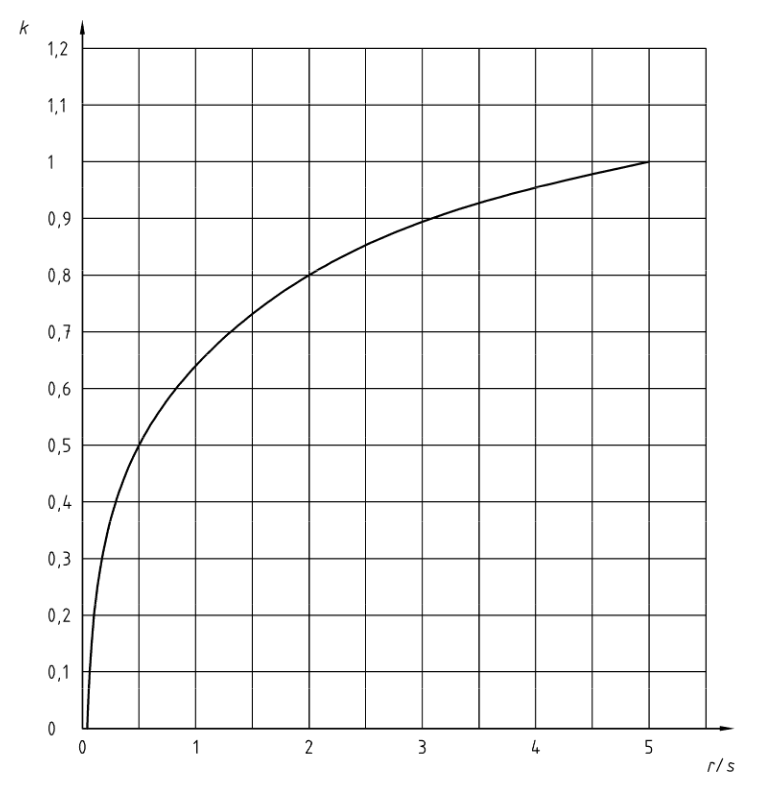
\includegraphics[width=0.5\linewidth]{k-factor}
	\caption[Graphical representation of the correction factor]{Graphical representation of the correction factor.}
	\label{fig:test1}
\end{figure}

The DIN 6935 used the formula for the stretched length, $length=a+b+v$ where \textit{a} and \textit{b} are the side lengths of the sheet and \textit{v} is a correction value for the deduction. \cite{din6935}
The stretched length is measured different depending on the bending angle.

\paragraph{Opening angle $\beta 0^\circ$ to $90^\circ$} 
For opening angles between $0^\circ$and $90^\circ$ the side lengths \textit{a} and \textit{b} are dimensioned from the tangent of the bend to the edge. 
To calculate the compensation value \textit{v} (Equation~\ref{eq:v1}) is used
\cite{din6935}.

\begin{equation}\label{eq:v1}
        v=\pi*(\frac{180^\circ-}{180^\circ})*(r+\frac{s}{2}*k)-2(r+s)
\end{equation}

\begin{figure}[H]
	\centering
	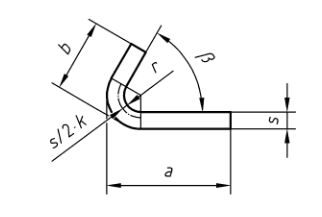
\includegraphics[width=0.5\linewidth]{bending-angle-90}
	\caption[Opening angles $\beta 0^\circ$ to $90^\circ$]{Opening angles $\beta 0^\circ$ to $90^\circ$ \cite{din6935}}
	\label{fig:v1-image}
\end{figure}

\paragraph{Bending angle $\beta90^\circ$ to $165^\circ$} (Equation~\ref{eq:v1})
For opening angles between $90^\circ$ and $165^\circ$ the side lengths \textit{a} and \textit{b} are dimensioned from the apex to the edge. 
To calculate the compensation value \textit{v} (Equation~\ref{eq:v1}) is used. 
\cite{din6935}

\begin{equation}\label{eq:v2}
    v=\pi*(\frac{180^\circ-}{180^\circ})*(r+\frac{s}{2}*k)-2(r+s)+\tan{\frac{180^\circ-\beta}{2}}
\end{equation}

\begin{figure}[!h]
	\centering
	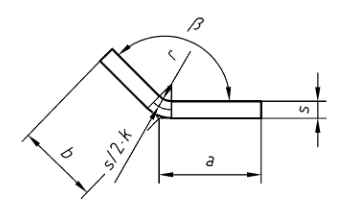
\includegraphics[width=0.5\linewidth]{bending-angle-165}
	\caption[Opening angles $\beta90^\circ$ to $165^\circ$]{Opening angles $\beta90^\circ$ to $165^\circ$ \cite{din6935}}
	\label{fig:v2-image}
\end{figure}

For opening angles between $165^\circ$ and $180^\circ$ the compensation value \textit{v} is 0. The values for v would be negligibly small. \cite{din6935} The side lengths \textit{a} and \textit{b} where measured using the software \textit{ImageJ}. 

Edge cracking is not measured for now because the steel used has no high-strength and with machine in usage it was not possible to create edge cracking.

\begin{figure}[!h]
	\centering
	\includegraphics[width=0.5\linewidth]{example-image}
	\caption[Screenshot ImageJ]{Screenshot ImageJ}
	\label{fig:imagej-screenshot}
\end{figure}



\begin{table}[ht!]
\centering
    \begin{tabular}{ |c|c|c|c| } 
        \hline
        Parameters & Mechanical Press \\
        \hline
        Load Tonnage (T) & tbd... \\
        Material & JSC440, JSC590, JSH440, JSH590 \\
        Thickness of blank (s) & 1.0 mm, 1.2 mm, 1.4 mm, 1.6 mm \\ 
        dimensions of plate (w) & 50 mm, 100 mm \\ 
        Bend angle & 60, 90 and 120 \\
        \hline
    \end{tabular}
    \caption{Parameters for the experimental setup}
\end{table}


    \input{chap4/results_and_discussion_main}
%%	\part{Your Second Part}
    \input{chap5/evaluation_main}
    \input{chap6/conclusions_main}
    \appendix
        \input{appA/appendix_a_main}     % these are just test names as I didn't know what you'd want
        \input{appB/appendix_b_main}    
        \input{appC/appendix_c_main} 

\pagestyle{umpageback}
{\backmatter
    % Bibliography
    \if@openright\cleardoublepage\else\clearpage\fi

    \bibliographystyle{um-plainnat} %% specific plainnat does not show url for articles
    % Use something like https://flamingtempura.github.io/bibtex-tidy/ to clean all your bibtex entries
    { 	\scriptsize\bibliography{
    chap1/introduction_biblio,
    chap2/background_and_lit_overview_biblio,
    chap2/theoretical_foundations_biblio,
    chap3/research_methodology_biblio 
    }}
	\printindex
}

\end{document}

%%% The End %%%
